\documentclass[a4paper,12pt]{article}

\usepackage[T1]{fontenc}
\usepackage[utf8]{inputenc}
\usepackage[francais]{babel}
\usepackage{multirow,array}
\usepackage{graphicx}
\usepackage{a4wide}
\newcommand{\HRule}{\rule{\linewidth}{1mm}}

\begin{document}


%
%  TITRE
%

\begin{titlepage}

\begin{center}
\huge Tables de hashage dynamiques et adaptatives pour une indexation en mémoire générique et souple des maillages.
\HRule \\
\medskip
{\Huge \bfseries La librairie libHash} \\
\HRule
\end{center}

\vspace*{\stretch{3}}

\begin{figure}[htbp]
\begin{center}
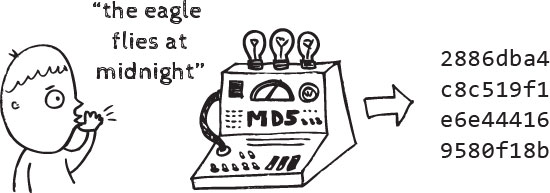
\includegraphics[width=14cm]{eagle.jpg}
\end{center}
\end{figure}

\vspace*{\stretch{1}}

\begin{flushright}
\Large Lo\"ic MAR\'ECHAL / INRIA, Projet Gamma\\
\Large Juin 2019 \\
\normalsize Document v1.0
\normalsize Librairie v1.4
\end{flushright}

\end{titlepage}

\clearpage

\setcounter{tocdepth}{2}
\tableofcontents
\vfill

\footnotesize{Couverture : ROB SOBERS, "The Definitive Guide to Cryptographic Hash Functions"}
\normalsize

\clearpage


%
%  1 / INTRODUCTION
%

\section{Introduction}

La libHash est une librairie permettant d'indexer des maillages via une table de hashage et de rechercher des entités selon des critères librement définis par le programmeur et cela en temps constant, quelle que soit la taille du maillage.
L'idée principale est d'associer des paires élément / sommet que l'on ajoute à la table de hashage, puis d'effectuer des requêtes en précisant un ou plusieurs sommets et la librairie retournera la liste des éléments référençant tous les sommets demandés.

Il est par exemple très simple d'ajouter tous les tétraèdres d'un maillage à une table de hashage puis d'effectuer des requêtes sur un seul numéro de sommet, ce qui retournera la boule de ce sommet, ou bien en fournissant deux sommets comme requête, ce qui retournera la coquille de l'arrête définie par ces deux sommets.

Le type de requêtes n'est limité que par l'imagination du programmeur !

La librairie a été implémentée dans un souci de simplicité pour le programmeur et de compacité mémoire, au détriment parfois des performances.
La taille des tables de hashage est gérée dynamiquement par la librairie et augmente ou diminue en fonction du nombre d'entités ajoutées ou retirées à une table.
Bien qu'une liste d'éléments types soit fournie (arrête, triangles, tétraèdre, etc.), l'utilisateur peut aussi ajouter les siennes.
Il n'y a pas de limite au nombre de sommets servant de clef de recherche et on peut tout à fait imaginer des usages où l'utilisation d'une dizaine de clefs aurait un sens.

Enfin, la fonction de requête de cette librairie est \emph{thread-safe}, et il est possible d'effectuer des recherches en parallèle à partir de différents threads.
La construction de la table de hashage reste par contre séquentielle.


%
%  2 / UTILISATION
%

\section{Utilisation}

La libHash est composée d'un fichier en langage C et d'un include et l'intégration dans votre code consiste simplement à ajouter ces deux fichiers à votre projet et à les compiler en même temps.
Par défaut, les entiers servant à passer les numéros des entités de maillage sont stockés sur 32 bits, mais il est possible d'étendre cette taille à 64 bits en compilant la librairie avec le paramètre -DINT64 à passer au compilateur.

Il faut tout d'abord initialiser une nouvelle table de hashage avec la commande \\
hsh\_NewTable() qui ne prend tout simplement aucun paramètre et se contente de retourner une étiquette sur la table nouvellement créée.
Cette étiquette sera demandée à chaque appel de commande de la librairie afin de différencier parmi toutes les tables allouées (sans limite).

Puis on va remplir la table à l'aide de la fonction hsh\_AddItem(), à laquelle on précise un numéro de table de destination, un type d'élément et une paire élément/sommet.

Une fois la table remplie, on peut effectuer des requêtes via hsh\_GetItem() en précisant le type d'élément recherché et la liste de sommets que les éléments doivent contenir pour répondre au critère de recherche.
La librairie va alors retourner le nombre et la liste des éléments concernés, et ce, en temps constant, quelle que soit la taille de la table de hashage.
On peut tout à fait modifier la table en ajoutant ou retirant des entités en cours de route et continuer à faire des requêtes entre temps.
Ces requêtes peuvent être effectuées de manière concurrente par plusieurs threads à condition de passer le numéro du thread appelant à la procédure hsh\_GetItem().

Enfin, un simple appel à hsh\_FreeTable() libère toute la mémoire prise par cette table uniquement.


%
%  3 / COMMANDES
%

\section{Liste des commandes}


\subsection{hsh\_NewTable}
Création d'une nouvelle table de hashage générique.
La taille de la table étant adaptative et le nombre de clefs variable, aucun argument n'est donc nécessaire.

\subsubsection*{Syntaxe}
{\tt Table = hsh\_NewTable();}

\subsubsection*{Commentaires}
Retourne une étiquette unique identifiant la table et qui devra être passé à toutes les autres fonctions.


\subsection{hsh\_FreeTable}
Libère toute la mémoire prise par une table et retourne le nombre d'octets occupés par la table ou 0 en cas d'echec.

\subsubsection*{Syntaxe}
Taille = hsh\_FreeTable(Table);

\subsubsection*{Paramètres}
\paragraph{Table:} l'index retourné par hsh\_NewTable() doit être passé.


\subsection{hsh\_AddItem}

\subsubsection*{Syntaxe}
{\tt flag = hsh\_AddItem(Table, type, Vertex, Élément, Unicité);}

\subsubsection*{Paramètres}
\begin{tabular}{|m{3cm}|m{2cm}|m{8.5cm}|}
\hline
Paramètre  & type     & description \\
\hline
Table      & int64\_t  & index de la table de hashage retournée par hsh\_NewTable \\
\hline
type       & int      & type de l'entité à ajouter à choisir dans les étiquettes prédéfinies ou bien librement \\
\hline
Vertex     & int      & Numéro du sommet par lequel cet élément est indexé \\
\hline
Élément    & int      & Numéro de l'entité à ajouter à la table de hash \\
\hline
Unicité    & int      & Flag valant 1 si on souhaite que chaque paire élément/sommet soir unique ou 0 si l'on accepte les doublons \\
\hline
\end{tabular}

\medskip

\begin{tabular}{|m{3cm}|m{2cm}|m{8.5cm}|}
\hline
Retour     & type   & description \\
\hline
index      & int    & retourne 1 en cas de succès ou 0 si la paire élément/sommet était déjà présente \\
\hline
\end{tabular}

\subsubsection*{Commentaires}
Un même élément peut être indexé plusieurs fois par plusieurs sommets (par exemple ajouter quatre fois un tétraèdre à la table de hash via ses quatre sommets).
Cela permet par la suite de retrouver ce tétraèdre en effectuant une requête sur une seule clef (boule d'un point), de deux clefs (coquille d'arrête) ou bien de trois (voisinage par face).

\subsubsection*{Exemple}

\begin{tt}
\begin{verbatim}
for(i=1;i<=NmbTet;i++)
  for(j=0;j<4;j++)
    hsh_AddItem(HshIdx, HshTet, TetTab[i][j], i, 1);
\end{verbatim}
\end{tt}
\normalfont

Boucle sur tous les tétraèdres du maillage, puis pour chaque élément, boucle sur ses quatre sommets et l'ajoute à la table autant de fois.


\subsection{hsh\_DeleteItem}

\subsubsection*{Syntaxe}
{\tt flag = hsh\_DeleteItem(table, type, Vertex, Élément);}

\subsubsection*{Paramètres}
\begin{tabular}{|m{3cm}|m{2cm}|m{8.5cm}|}
\hline
Paramètre  & type     & description \\
\hline
Table      & int64\_t  & index de la table de hashage retournée par hsh\_NewTable \\
\hline
type       & int      & type de l'entité à ajouter à choisir dans les étiquettes prédéfinies ou bien librement \\
\hline
Vertex     & int      & Numéro du sommet par lequel cet élément est indexé \\
\hline
Élément    & int      & Numéro de l'entité à supprimer à la table de hash \\
\hline
\end{tabular}

\subsubsection*{Commentaires}
La mémoire étant allouée par bloc de 10.000 entités, elle ne sera effectivement libérée que lorsque tous les éléments contenus dans un bloc auront été supprimés par hsh\_DeleteItem().
Comme il n'y a pas de "garbage collector", l'effet gruyère peut entrainer une mauvaise efficacité de l'utilisation mémoire.

\medskip

\begin{tabular}{|m{3cm}|m{2cm}|m{8.5cm}|}
\hline
Retour     & type   & description \\
\hline
index      & int    & retourne 1 si la paire élément/sommet a été trouvée et effacée ou 0 en cas s'échec \\
\hline
\end{tabular}

\subsubsection*{Exemple}

\begin{tt}
\begin{verbatim}
hsh_DeleteItem(HshIdx, HshPyr, 115, 8);
\end{verbatim}
\end{tt}
\normalfont

Retire la pyramide numéro 115 hashée selon le sommet 8.


\subsection{hsh\_GetItem}

\subsubsection*{Syntaxe}
{\tt flag = itg hsh\_GetItem(table, thread, type, nombreVertex, tableVertices, tableElements, tableTypes);}

\subsubsection*{Paramètres}
\begin{tabular}{|m{3cm}|m{2cm}|m{8.5cm}|}
\hline
Paramètre     & type     & description \\
\hline
Table         & int64\_t & index de la table de hashage retournée par hsh\_NewTable \\
\hline
thread        & int      & numéro du thread appelant cette routine dans le cas d'exécution parallèle, ou 0 en mode séquentiel \\
\hline
type          & int      & type des entités à rechercher dans la table de hash \\
\hline
nombreVertex  & int      & nombre de sommets de tableVertices à fournir à la suite \\
\hline
tableVertices & int *    & tableau d'entier contenant les index de sommets qui serviront de clef de hashage \\
\hline
tableElements & int *    & tableau des éléments répondant à cette clef et renseigné par la procédure \\
\hline
tableTypes    & int *    & tableau optionnel contenant le type de chaque élément retourné \\
\hline
\end{tabular}

\medskip

\begin{tabular}{|m{3cm}|m{2cm}|m{8.5cm}|}
\hline
Retour     & type   & description \\
\hline
index      & int    & retourne le nombre d'éléments trouvés et écrit dans la tableElements \\
\hline
\end{tabular}

\subsubsection*{Commentaires}
Cette fonction très puissante permet d'effectuer plusieurs types de recherches dans une base de données de maillage via une procédure unique.
Le comportement est identique, mais le sens change en fonction du nombre de sommets sur lesquels on base la requête.

Un sommet : retourne la liste des éléments partageant ce sommet, il s'agit le sa boule.
Deux sommets : retourne la liste des éléments partageant l'arrête définie par ces deux sommets, il s'agit de sa coquille.
Trois ou quatre sommets : retourne les deux éléments partageant la même face définie par ces triangle ou quadrilatère, il s'agit du voisinage par face.

\subsubsection*{Exemple}

\begin{tt}
\begin{verbatim}
for(i=1;i<=NmbTet;i++)
  for(j=0;j<4;j++)
  {
    for(k=0;k<3;k++)
      VerFac[k] = TetTab[i][ tettvpf[j][k] ];
    
    if(hsh_GetItem(HshIdx, 0, HshAny, 3, VerFac, &EleTab, NULL) == 1)
      NmbTri++;
  }
\end{verbatim}
\end{tt}
\normalfont

Boucle sur tous les tétraèdres, boucle sur les quatre faces de chaque élément, remplie une table VerFac contenant les indices des trois sommets de cette face et effectue une requête à la table hashage.
Si le nombre d'éléments trouvé est égal à 1, cela veut dire que cette face de tétraèdre est sur la frontière et on incrémente le compteur de triangles.
Ce petit code permet de retrouver le nombre de triangles frontière à partir d'un maillage contenant seulement les tétraèdres du volume.

\end{document}
